\documentclass[11pt]{article}\usepackage[]{graphicx}\usepackage[]{color}
%% maxwidth is the original width if it is less than linewidth
%% otherwise use linewidth (to make sure the graphics do not exceed the margin)
\makeatletter
\def\maxwidth{ %
  \ifdim\Gin@nat@width>\linewidth
    \linewidth
  \else
    \Gin@nat@width
  \fi
}
\makeatother

\definecolor{fgcolor}{rgb}{0.345, 0.345, 0.345}
\newcommand{\hlnum}[1]{\textcolor[rgb]{0.686,0.059,0.569}{#1}}%
\newcommand{\hlstr}[1]{\textcolor[rgb]{0.192,0.494,0.8}{#1}}%
\newcommand{\hlcom}[1]{\textcolor[rgb]{0.678,0.584,0.686}{\textit{#1}}}%
\newcommand{\hlopt}[1]{\textcolor[rgb]{0,0,0}{#1}}%
\newcommand{\hlstd}[1]{\textcolor[rgb]{0.345,0.345,0.345}{#1}}%
\newcommand{\hlkwa}[1]{\textcolor[rgb]{0.161,0.373,0.58}{\textbf{#1}}}%
\newcommand{\hlkwb}[1]{\textcolor[rgb]{0.69,0.353,0.396}{#1}}%
\newcommand{\hlkwc}[1]{\textcolor[rgb]{0.333,0.667,0.333}{#1}}%
\newcommand{\hlkwd}[1]{\textcolor[rgb]{0.737,0.353,0.396}{\textbf{#1}}}%

\usepackage{framed}
\makeatletter
\newenvironment{kframe}{%
 \def\at@end@of@kframe{}%
 \ifinner\ifhmode%
  \def\at@end@of@kframe{\end{minipage}}%
  \begin{minipage}{\columnwidth}%
 \fi\fi%
 \def\FrameCommand##1{\hskip\@totalleftmargin \hskip-\fboxsep
 \colorbox{shadecolor}{##1}\hskip-\fboxsep
     % There is no \\@totalrightmargin, so:
     \hskip-\linewidth \hskip-\@totalleftmargin \hskip\columnwidth}%
 \MakeFramed {\advance\hsize-\width
   \@totalleftmargin\z@ \linewidth\hsize
   \@setminipage}}%
 {\par\unskip\endMakeFramed%
 \at@end@of@kframe}
\makeatother

\definecolor{shadecolor}{rgb}{.97, .97, .97}
\definecolor{messagecolor}{rgb}{0, 0, 0}
\definecolor{warningcolor}{rgb}{1, 0, 1}
\definecolor{errorcolor}{rgb}{1, 0, 0}
\newenvironment{knitrout}{}{} % an empty environment to be redefined in TeX

\usepackage{alltt}
%---------------------------------------------------------------------%
% PROGRAM: Correlation_AUP513.Rnw
%
% DESCRIPTION: This code generates correlation plots for AUP513 manuscript.
%
% CODED BY: Bhavesh Borate on 1/4/2017
% PROJECT : AUP513 manuscript: Correlation between ICS and other assays
%
%
% MAINTENANCE HISTORY:
%   Date        Programmer       Description
%   1/4/2017    Bhavesh Borate   Version 0.1
%
%----------------------------------------------------------------------%
\usepackage{url}
\usepackage{float}
\usepackage{color, pdfcolmk}
\usepackage{natbib}
\renewcommand{\bibsection}{}
\usepackage[hmargin=2cm, vmargin=3cm]{geometry}
\usepackage{fancyhdr, graphicx, lastpage, ifthen, lscape, xcolor}
\usepackage{etoolbox}
\usepackage{pdflscape}
\usepackage[absolute]{textpos}
\usepackage{rotating} %for xtable sideways
\usepackage{verbatim}
\usepackage{longtable}
\usepackage{subfigure}
\usepackage{changepage}
\usepackage{chngcntr}
% \counterwithin{figure}{subsection}
% \counterwithin{table}{subsection}
\newcommand{\scscst}{\scriptscriptstyle}
\newcommand{\scst}{\scriptstyle}
\usepackage[font=normalsize,skip=4pt,justification=centering]{caption}
\usepackage[parfill]{parskip}
\usepackage[colorlinks=true,linkcolor=blue]{hyperref}
\usepackage{titlesec}
\usepackage{fixltx2e}

\setcounter{secnumdepth}{4}

\titleformat{\paragraph}
{\normalfont\normalsize\bfseries}{\theparagraph}{1em}{}
\titlespacing*{\paragraph}
{0pt}{3.25ex plus 1ex minus .2ex}{1.5ex plus .2ex}



\listfiles

\newcommand{\organiz}{SCHARP}
\newcommand{\uident}{bborate}
\newcommand{\Rver}{R version 3.2.1 }
\newcommand{\DynLength}{0.2}
%this is to adjust header and footer in landscaped pages
\fancypagestyle{lscape}{%
    \newgeometry{hmargin=1.0cm,vmargin=0.5cm}
    \fancyhf{} % clear all header and footer fields
    \fancyfoot[L]{
    \begin{textblock}{1}(21.12,1.75){\color{gray}\rotatebox{90}{Page \thepage{}~of~\pageref{LastPage}}}\end{textblock}}
    \fancyfoot[R]{
    \begin{textblock}{19.7}[-0.01,{\DynLength}](1.5,23.20){\color{gray}\rotatebox{90}{\Rver}}\end{textblock}}
    \setlength{\TPHorizModule}{1cm}
    \setlength{\TPVertModule}{1cm}
    \renewcommand{\headrulewidth}{0.0pt}
    \renewcommand{\footrulewidth}{0.0pt}}
%this is to adjust header and footer in regular pages
\fancypagestyle{regularpage}{
    \pagestyle{fancy}
    \newgeometry{textheight=624.25346pt,headheight=12.0pt,headsep=25.0pt,footskip=56.0pt,voffset=0.0pt,hmargin=2cm,vmargin=3cm}
    \fancyhf{}
    \renewcommand{\headrulewidth}{0.4pt}
    \renewcommand{\footrulewidth}{0.4pt}
    \fancyhead[L]{}
    \fancyhead[R]{\bfseries IPV 001ABMG}
    \fancyfoot[R]{Page \thepage{}~of~\pageref{LastPage}}
    \fancyfoot[L]{\Rver}}
%set header and footer for first page
\renewcommand{\headrulewidth}{0.8pt}
\renewcommand{\footrulewidth}{0.8pt}
\fancyhead[L]{ 
\includegraphics[height=1.25cm, width=5cm]{logos/scharp2.png}}
\fancyhead[R]{ 
\includegraphics[width=4cm]{logos/FredHutch_h_tag_4col_CMYK_tm.png} }
\fancyhead[C]{ 
\includegraphics[height=1.25cm, width=3cm]{logos/new_VISC_logo_color.jpg} }
\fancyfoot[C]{}
\fancyfoot[L]{\Rver}
\fancyfoot[R]{Page \thepage{}~of~\pageref{LastPage}}
%page settings
\setlength{\footskip}{56pt}
\pagestyle{fancy}
\IfFileExists{upquote.sty}{\usepackage{upquote}}{}
\begin{document}
\newcommand{\tab}{\hspace*{2cm}} %this sets length of horizontal space from tab
\newcommand{\bat}{\vspace*{2pc}} %this sets length of vertical space from tab
%font settings
\textnormal {\normalfont}
%get current date into insertdate
\makeatletter
\let\insertdate\@date
\makeatother

\bat
\Large \textbf{\\ AUP513: Correlation plots for manuscript} \\
\large
\insertdate \\ \\
\textbf{To:} Georgia Tomaras \\
\textbf{From:} Raphael Gottardo, Bhavesh Borate \\
\textbf{cc:} Alicia Sato, Eva Chung \\

\normalsize
\textbf{Overview} \\
This report presents the correlations between CD4/CD8 T-cell responses measured through ICS assay and the B-cell response measured through BAMA, GTL ADCC and NAb assays for the groups receiving NYVAC-C-KC vaccines (Groups 5 and 6). 

\listoffigures


\newpage
%change color of header and footer text to gray
\makeatletter
\patchcmd{\@fancyhead}{\rlap}{\color{gray}\rlap}{}{}
\patchcmd{\headrule}{\hrule}{\color{gray}\hrule}{}{}
\patchcmd{\@fancyfoot}{\rlap}{\color{gray}\rlap}{}{}
\patchcmd{\footrule}{\hrule}{\color{gray}\hrule}{}{}
\makeatother
%set header and footer for all pages from here
\newpage
\newgeometry{hmargin=2cm,vmargin=3cm}
\renewcommand{\headrulewidth}{0.4pt}
\renewcommand{\footrulewidth}{0.4pt}
\fancyhead[L]{}
\fancyhead[R]{\bfseries IPV 001ABMG}
\fancyfoot[R]{Page \thepage{}~of~\pageref{LastPage}}


% \makeatletter
% \renewcommand*\l@figure{\@dottedtocline{1}{1.5em}{3.0em}}
% \renewcommand*\l@table{\@dottedtocline{1}{1.5em}{3.0em}}
% \makeatother

\newpage
\pagestyle{lscape}
\begin{landscape}


%%%%%%%%%%%%%%%%%%%%%%%%%%%%%%%%%%%%%%%%%%%%%%%%%%%%%%%%%%%%%%%%%%%%%%%%%%%%%%%%%%%%%%%%%%%
%%%%%%%%%%%%%%%%%%%%%%%%%%%%%%%%%%%%%%%%%%%%%%%%%%%%%%%%%%%%%%%%%%%%%%%%%%%%%%%%%%%%%%%%%%%

% {\scriptsize
% \tab \textbf{Footnote: \newline}
% \tab *  -- Percentages in this group are computed using total number not enrolled as denominator. \newline
% \tab ** -- Percent enrolled is computed as fraction of N screened. Subsequent percentages in this group are computed as a fraction of N enrolled.\newline
% }



\begin{figure}[H]
\begin{center}
\begin{knitrout}
\definecolor{shadecolor}{rgb}{0.969, 0.969, 0.969}\color{fgcolor}
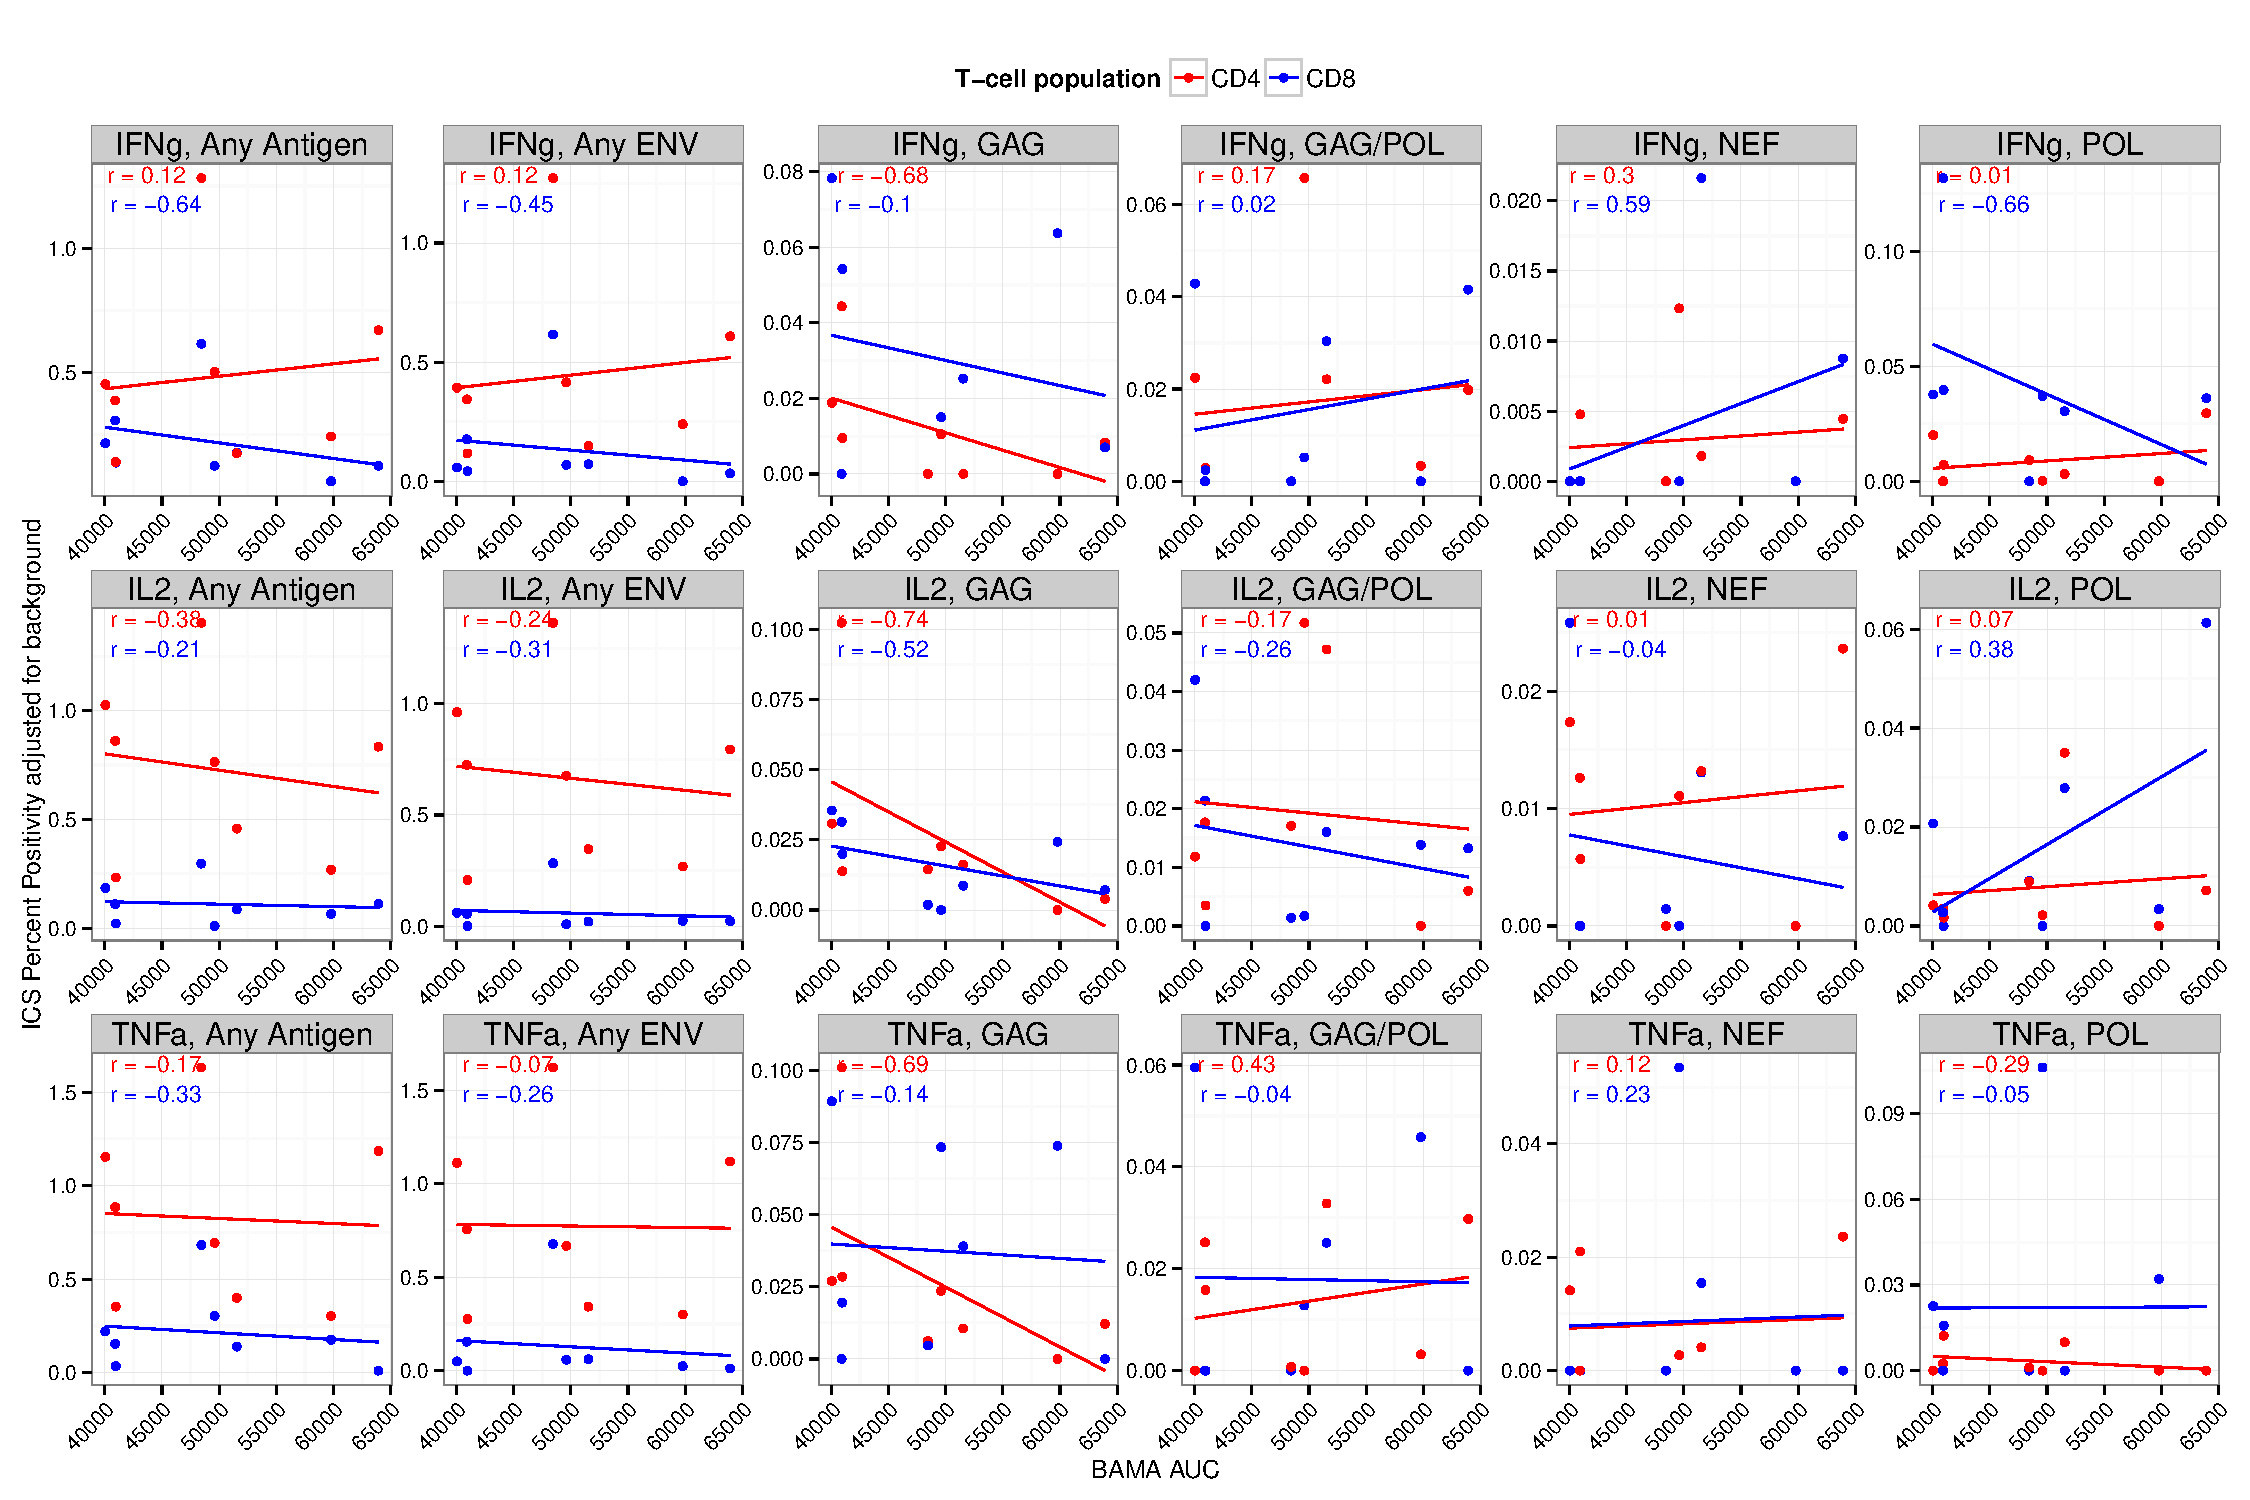
\includegraphics[width=\maxwidth]{figure/corrplot_Grp5_BAMA_pooledAntigen-1} 

\end{knitrout}
\caption{Group 5, ICS v/s BAMA by cytokine and pooled antigen colored by T-cell population. The fitted simple linear regression line and Spearman correlation are indicated.}
\end{center}
\end{figure}


\begin{figure}[H]
\begin{center}
\begin{knitrout}
\definecolor{shadecolor}{rgb}{0.969, 0.969, 0.969}\color{fgcolor}
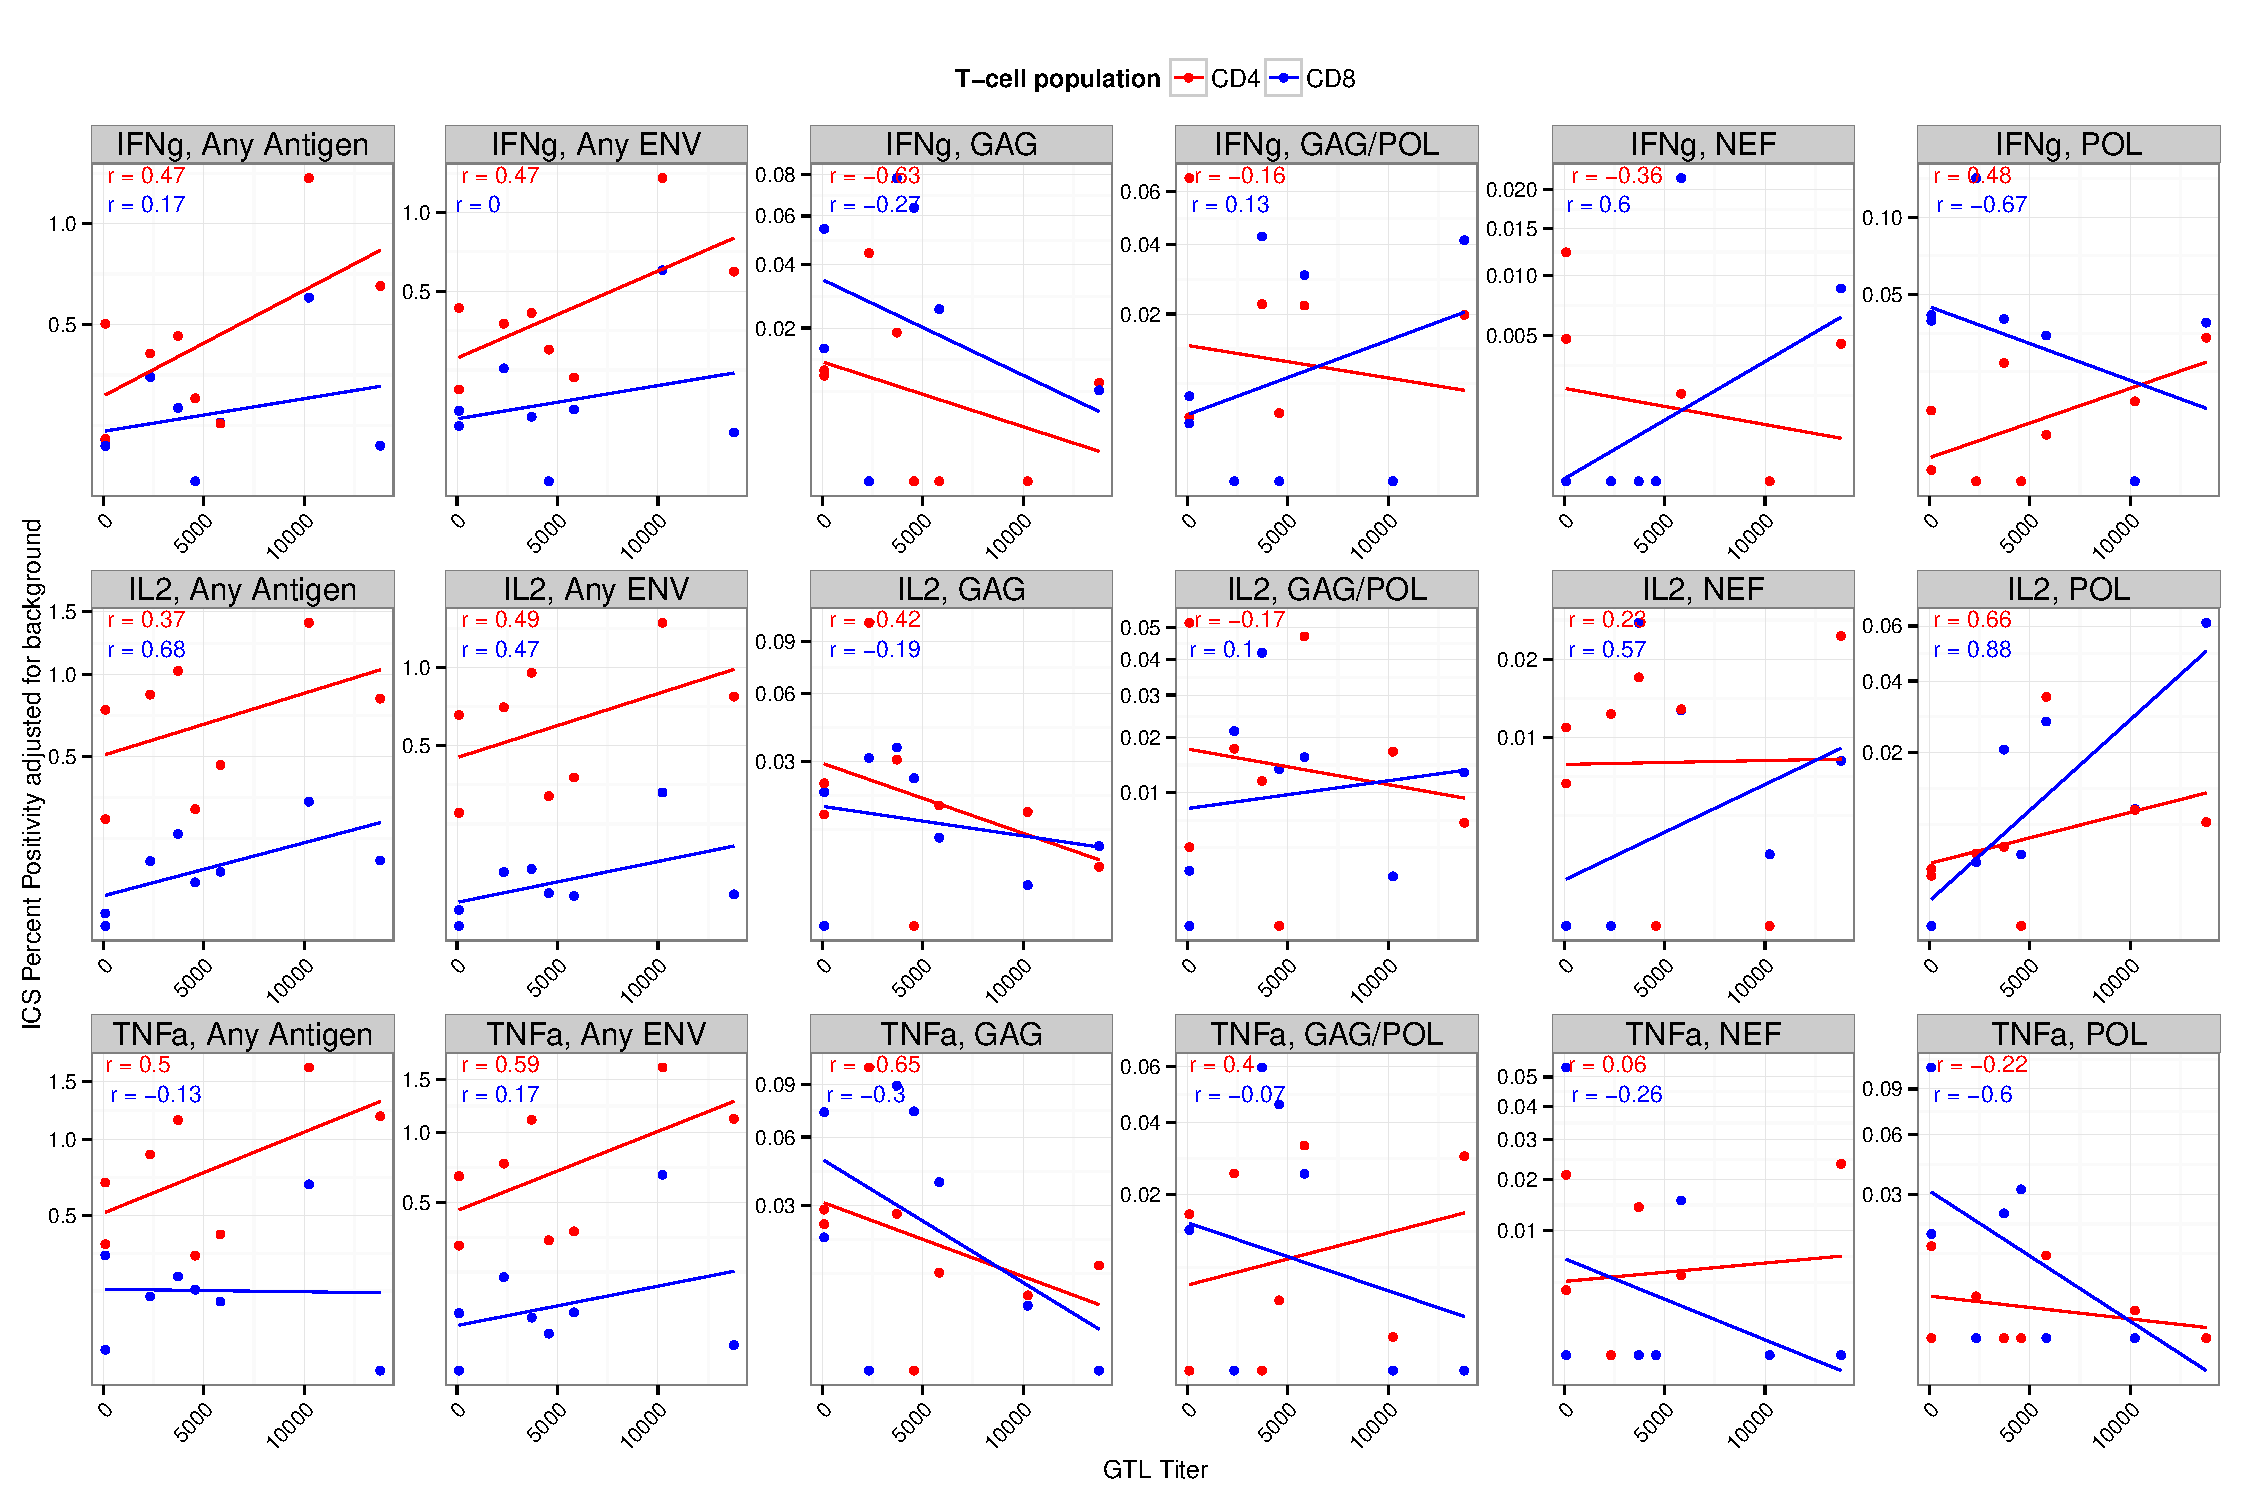
\includegraphics[width=\maxwidth]{figure/corrplot_Grp5_ADCC_pooledAntigen-1} 

\end{knitrout}
\caption{Group 5, ICS v/s ADCC GTL assay by cytokine and pooled antigen colored by T-cell population. The fitted simple linear regression line and Spearman correlation are indicated.}
\end{center}
\end{figure}


\begin{figure}[H]
\begin{center}
\begin{knitrout}
\definecolor{shadecolor}{rgb}{0.969, 0.969, 0.969}\color{fgcolor}
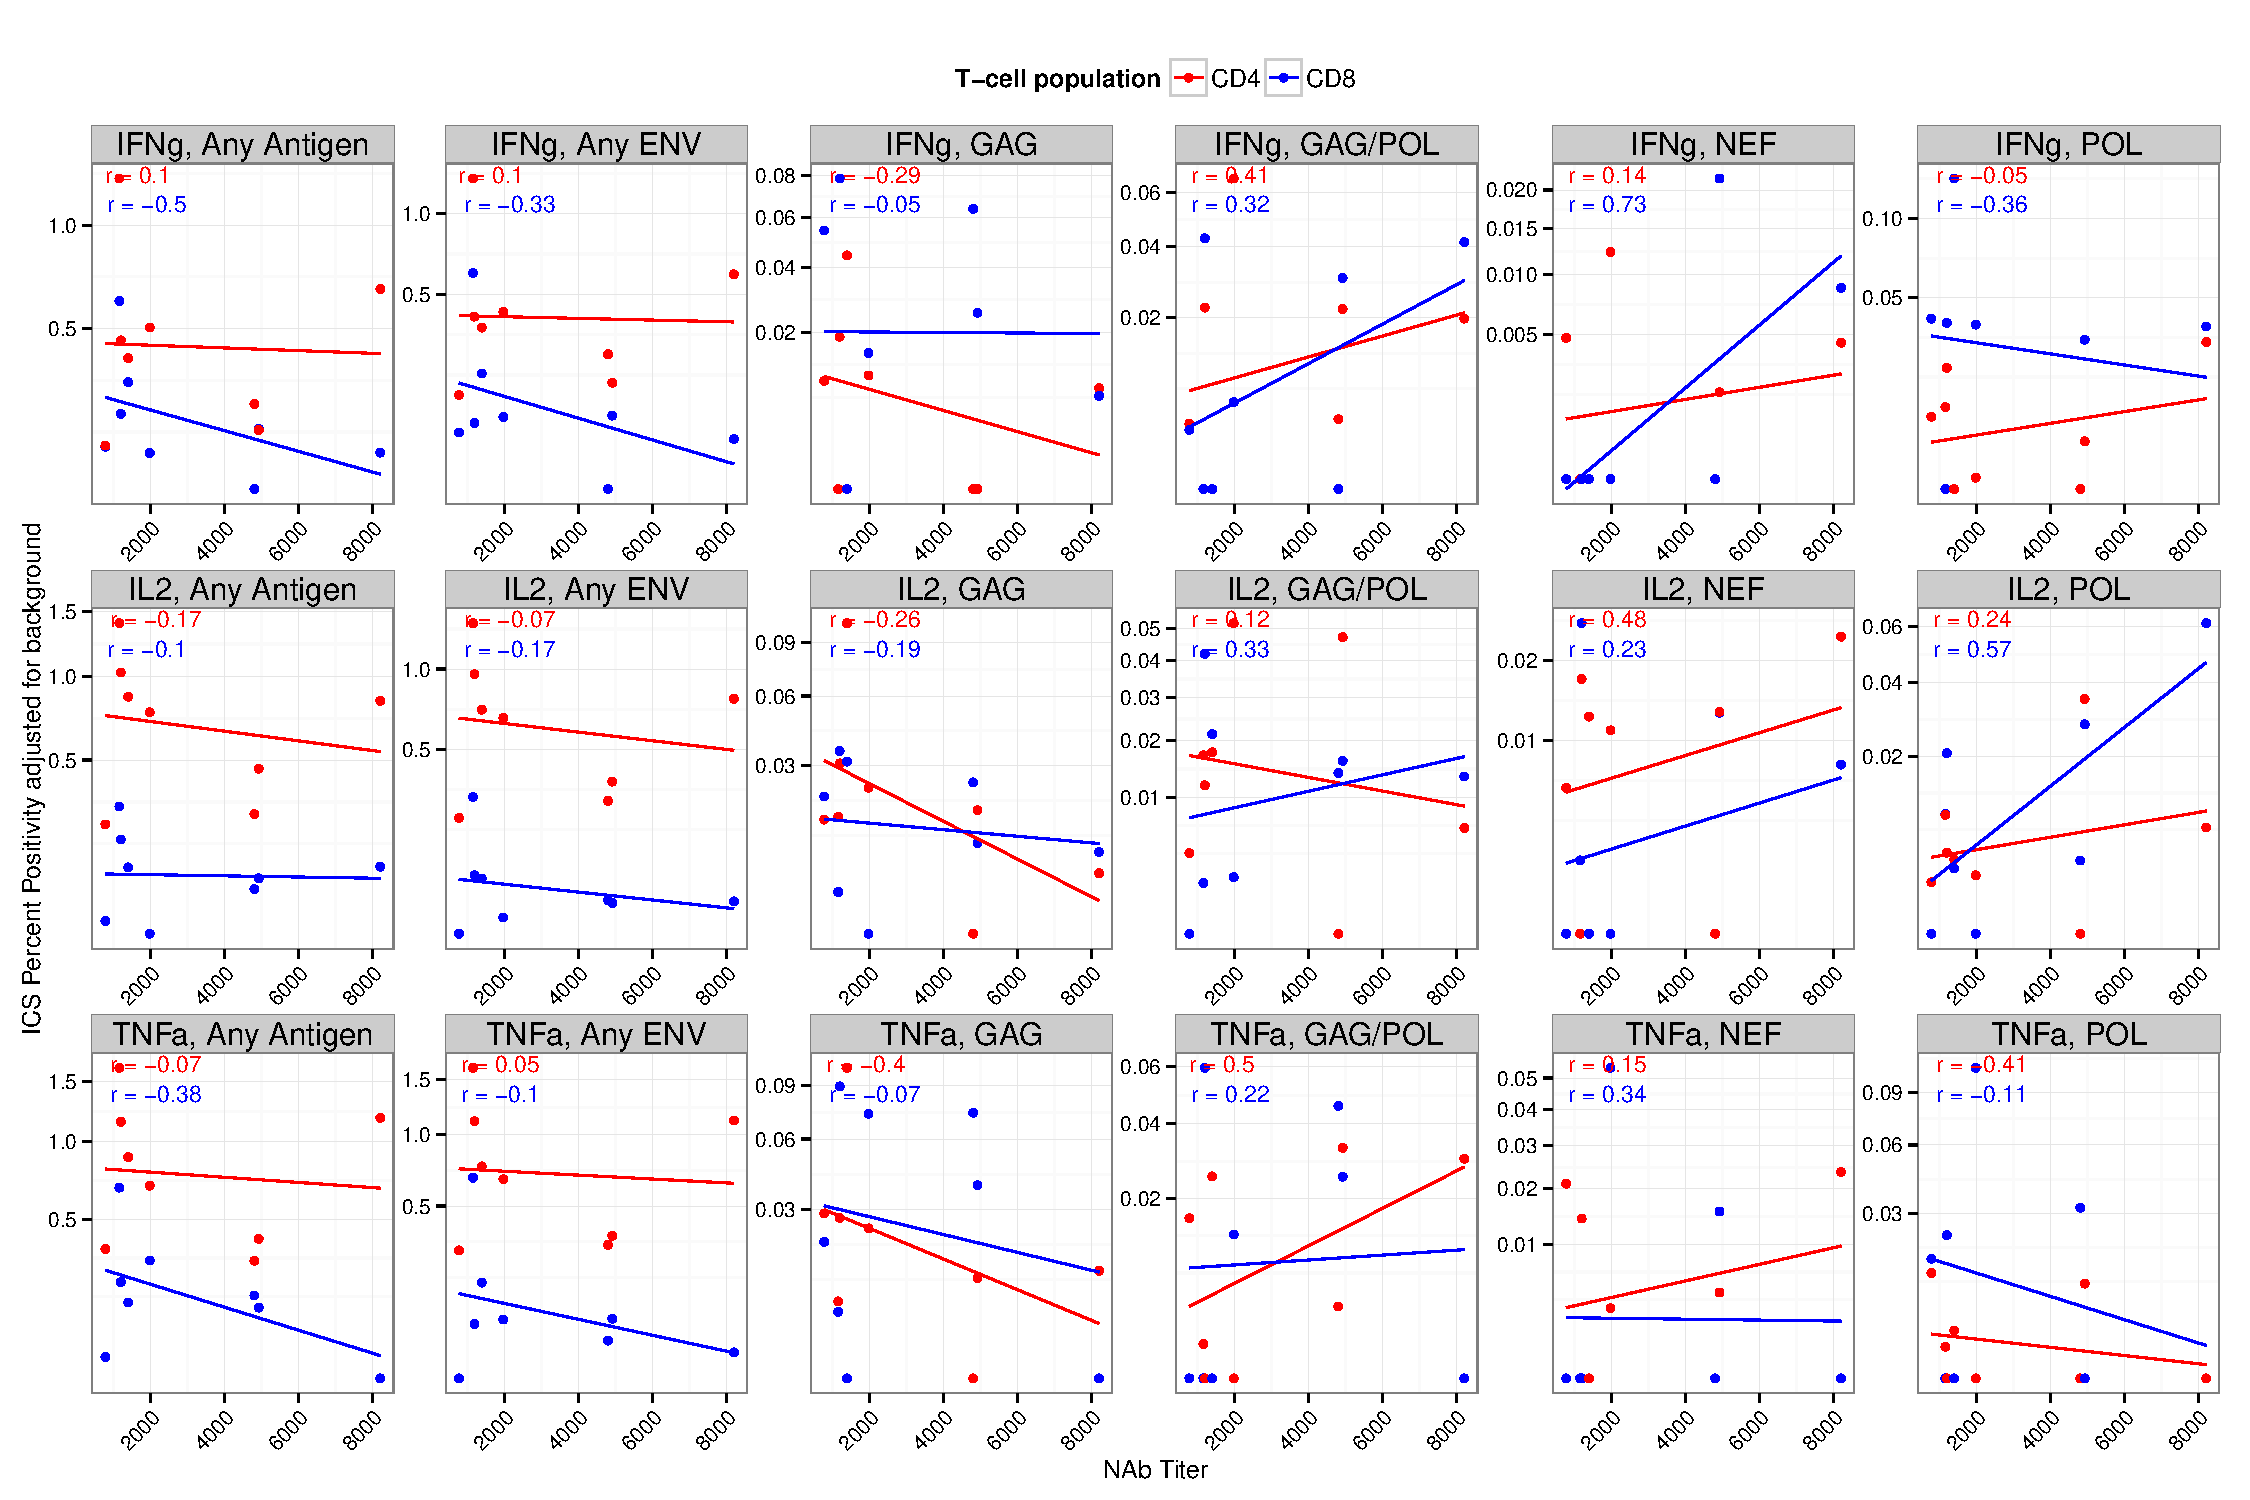
\includegraphics[width=\maxwidth]{figure/corrplot_Grp5_NAb_pooledAntigen-1} 

\end{knitrout}
\caption{Group 5, ICS v/s NAB assay by cytokine and pooled antigen colored by T-cell population. The fitted simple linear regression line and Spearman correlation are indicated.}
\end{center}
\end{figure}



\begin{figure}[H]
\begin{center}
\begin{knitrout}
\definecolor{shadecolor}{rgb}{0.969, 0.969, 0.969}\color{fgcolor}
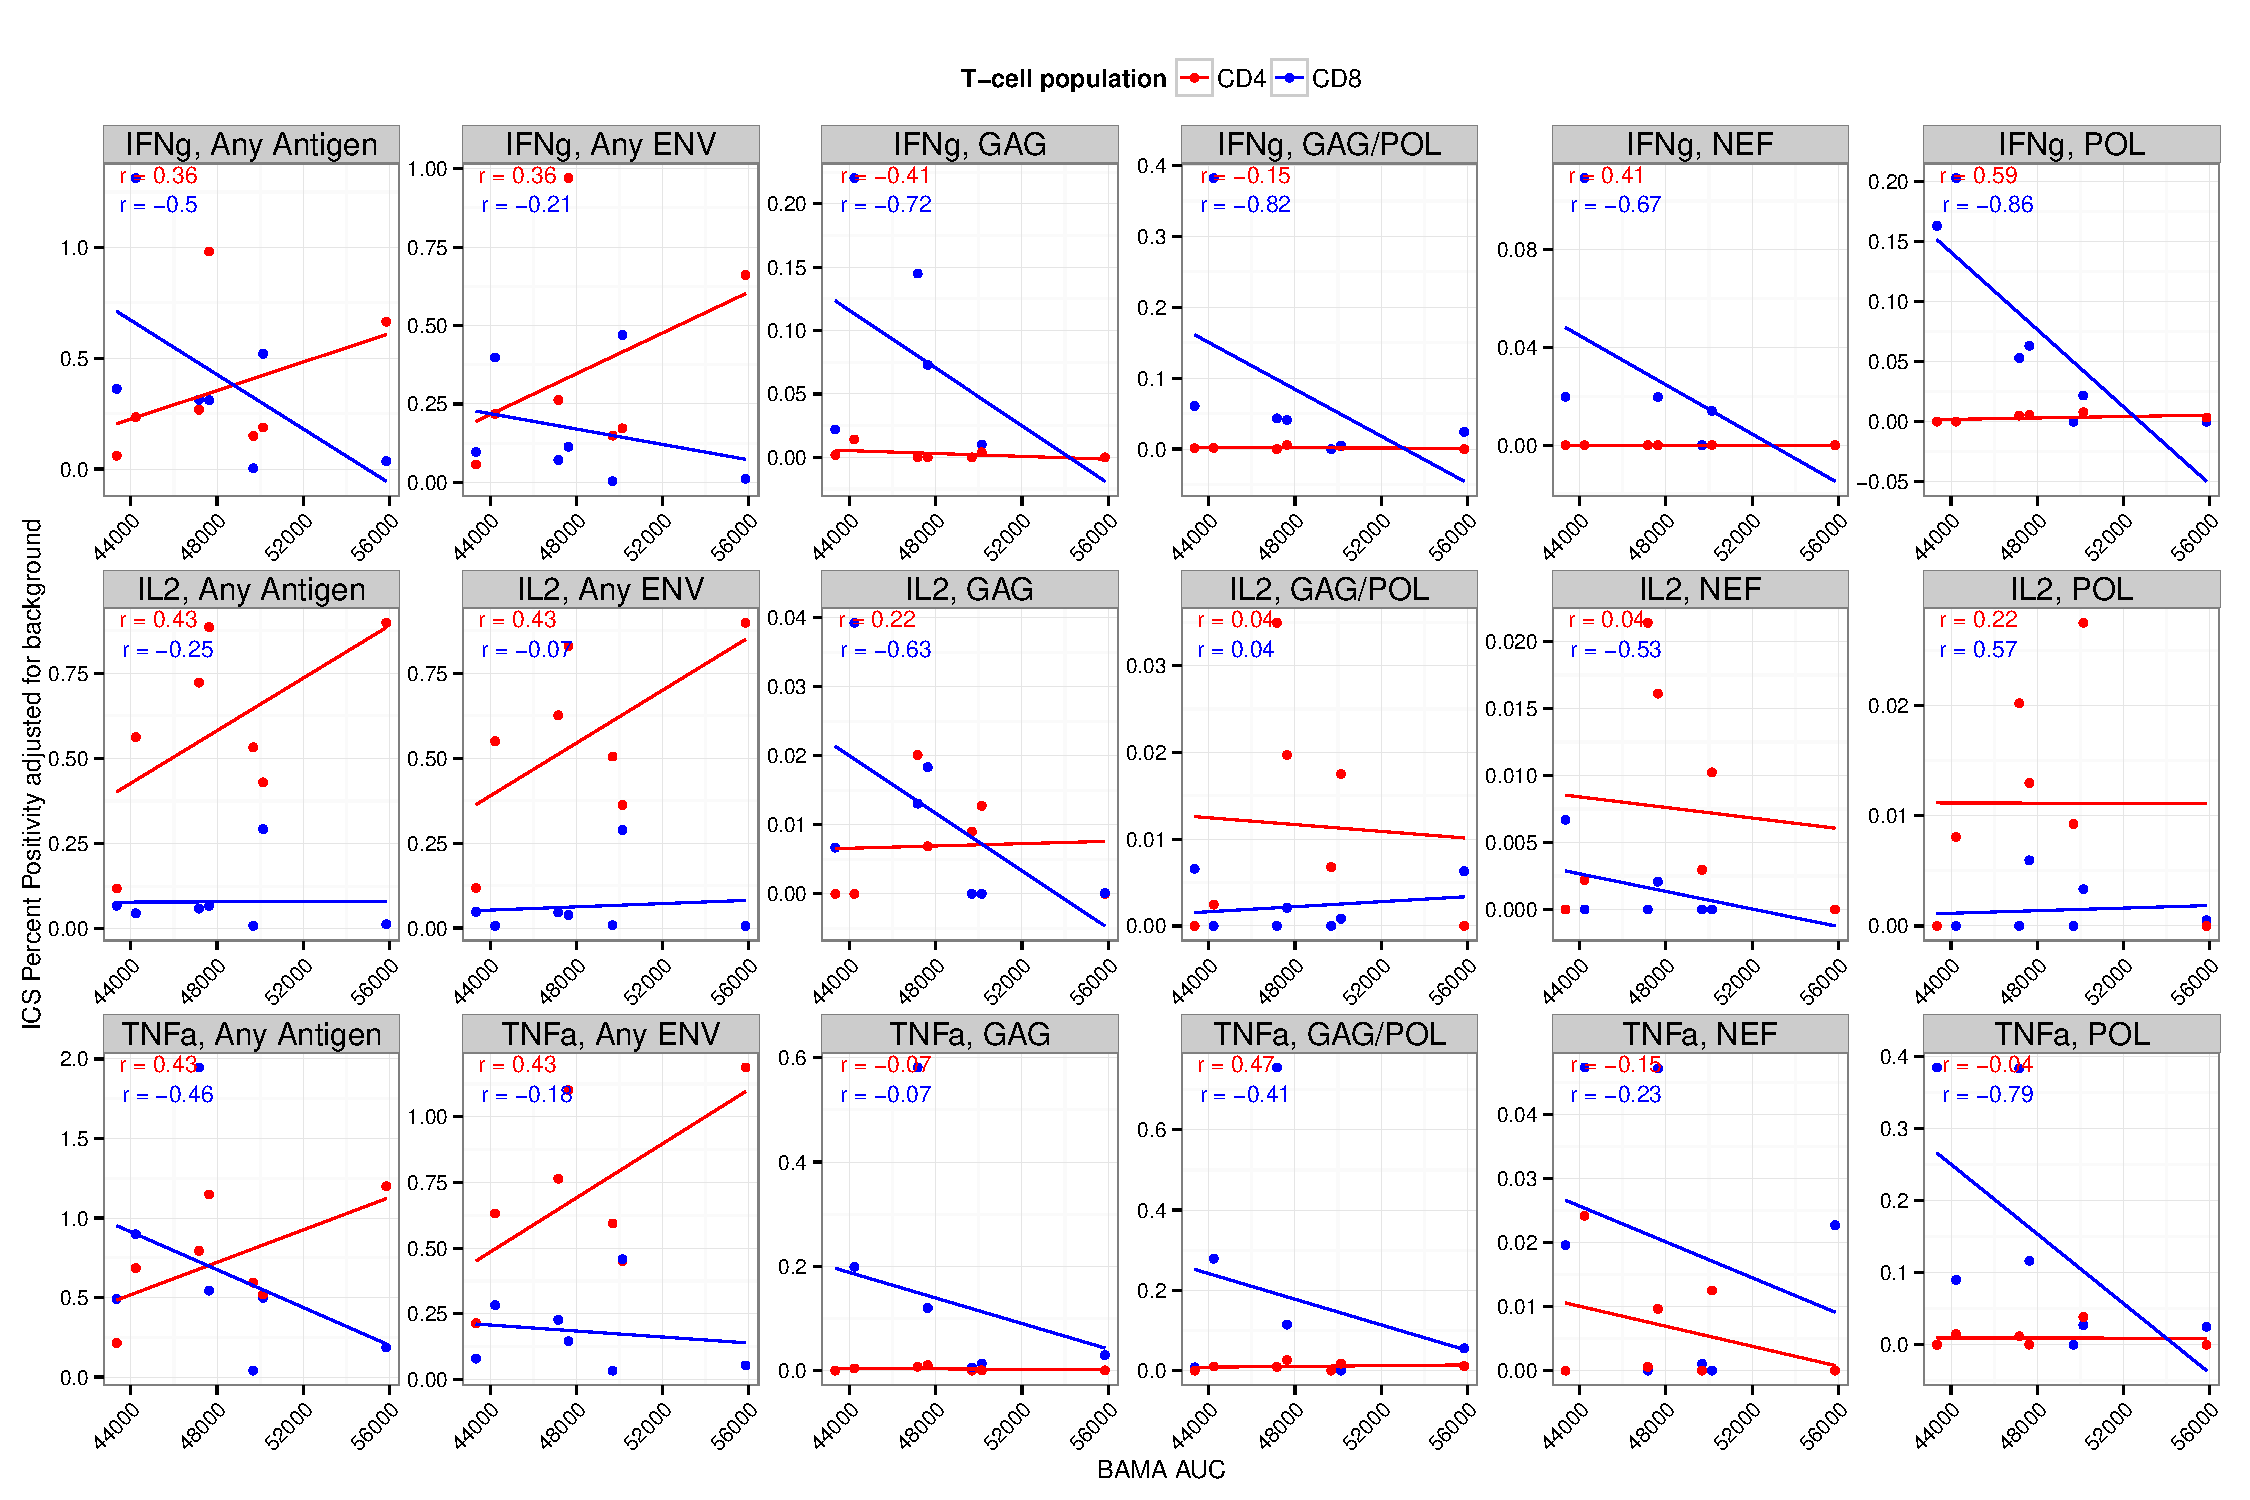
\includegraphics[width=\maxwidth]{figure/corrplot_Grp6_BAMA_pooledAntigen-1} 

\end{knitrout}
\caption{Group 6, ICS v/s BAMA by cytokine and pooled antigen colored by T-cell population. The fitted simple linear regression line and Spearman correlation are indicated.}
\end{center}
\end{figure}


\begin{figure}[H]
\begin{center}
\begin{knitrout}
\definecolor{shadecolor}{rgb}{0.969, 0.969, 0.969}\color{fgcolor}
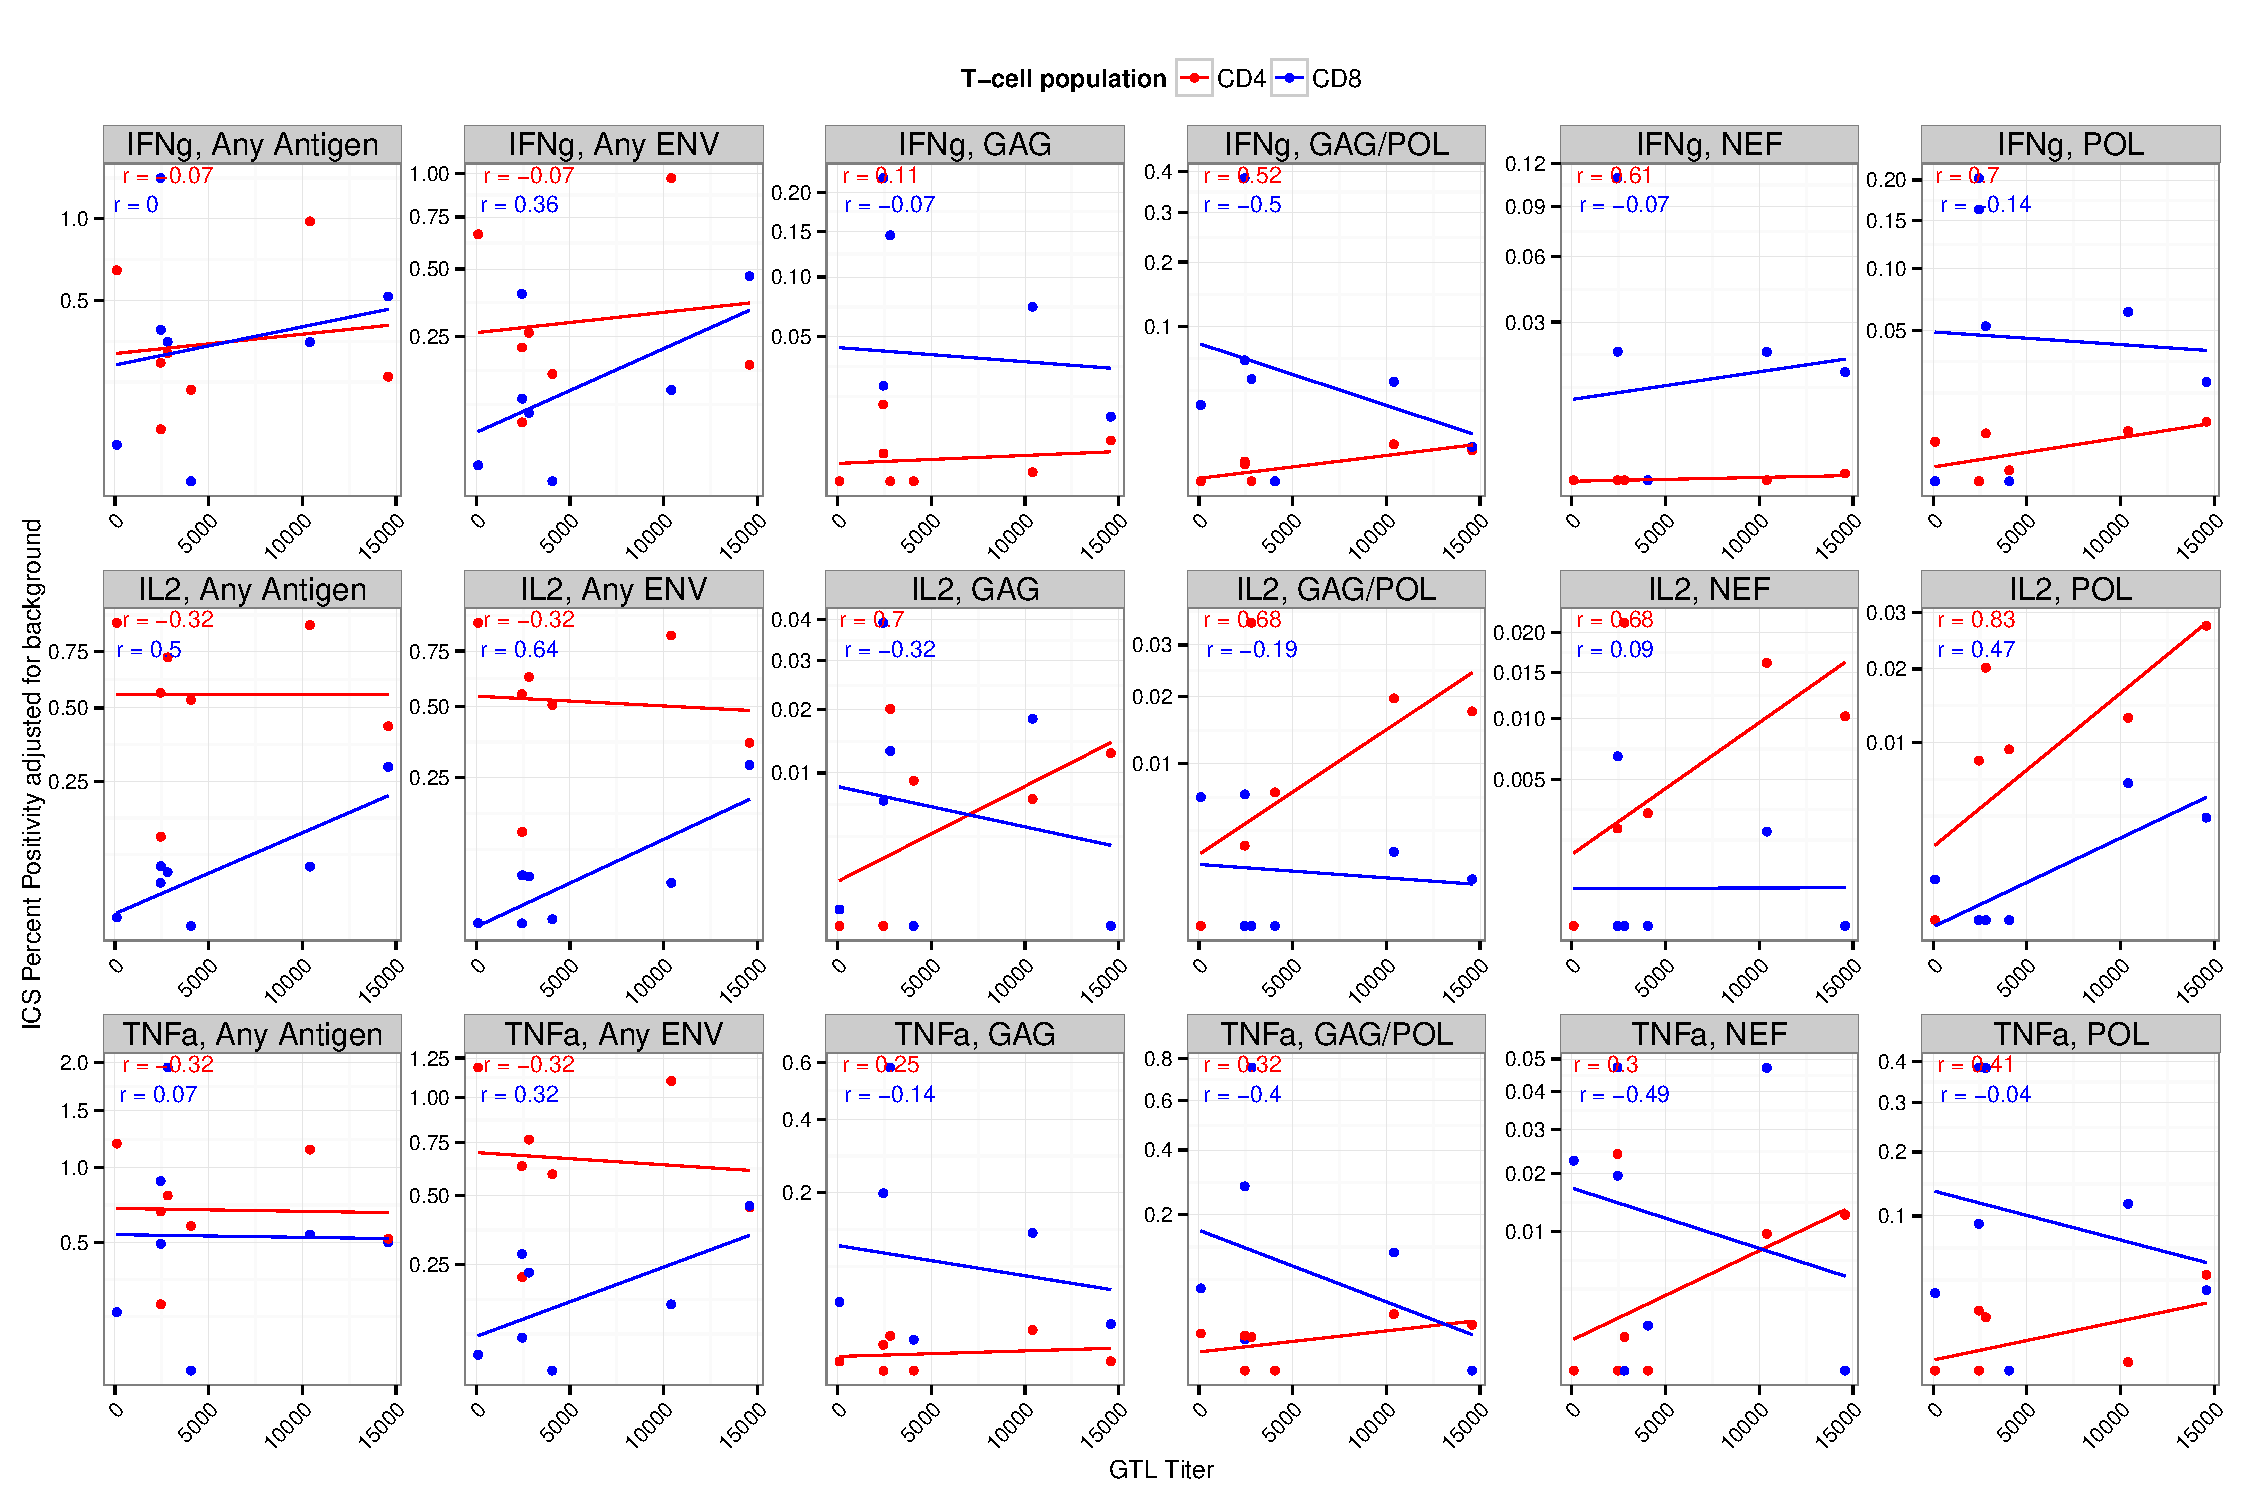
\includegraphics[width=\maxwidth]{figure/corrplot_Grp6_ADCC_pooledAntigen-1} 

\end{knitrout}
\caption{Group 6, ICS v/s ADCC GTL assay by cytokine and pooled antigen colored by T-cell population. The fitted simple linear regression line and Spearman correlation are indicated.}
\end{center}
\end{figure}


\begin{figure}[H]
\begin{center}
\begin{knitrout}
\definecolor{shadecolor}{rgb}{0.969, 0.969, 0.969}\color{fgcolor}
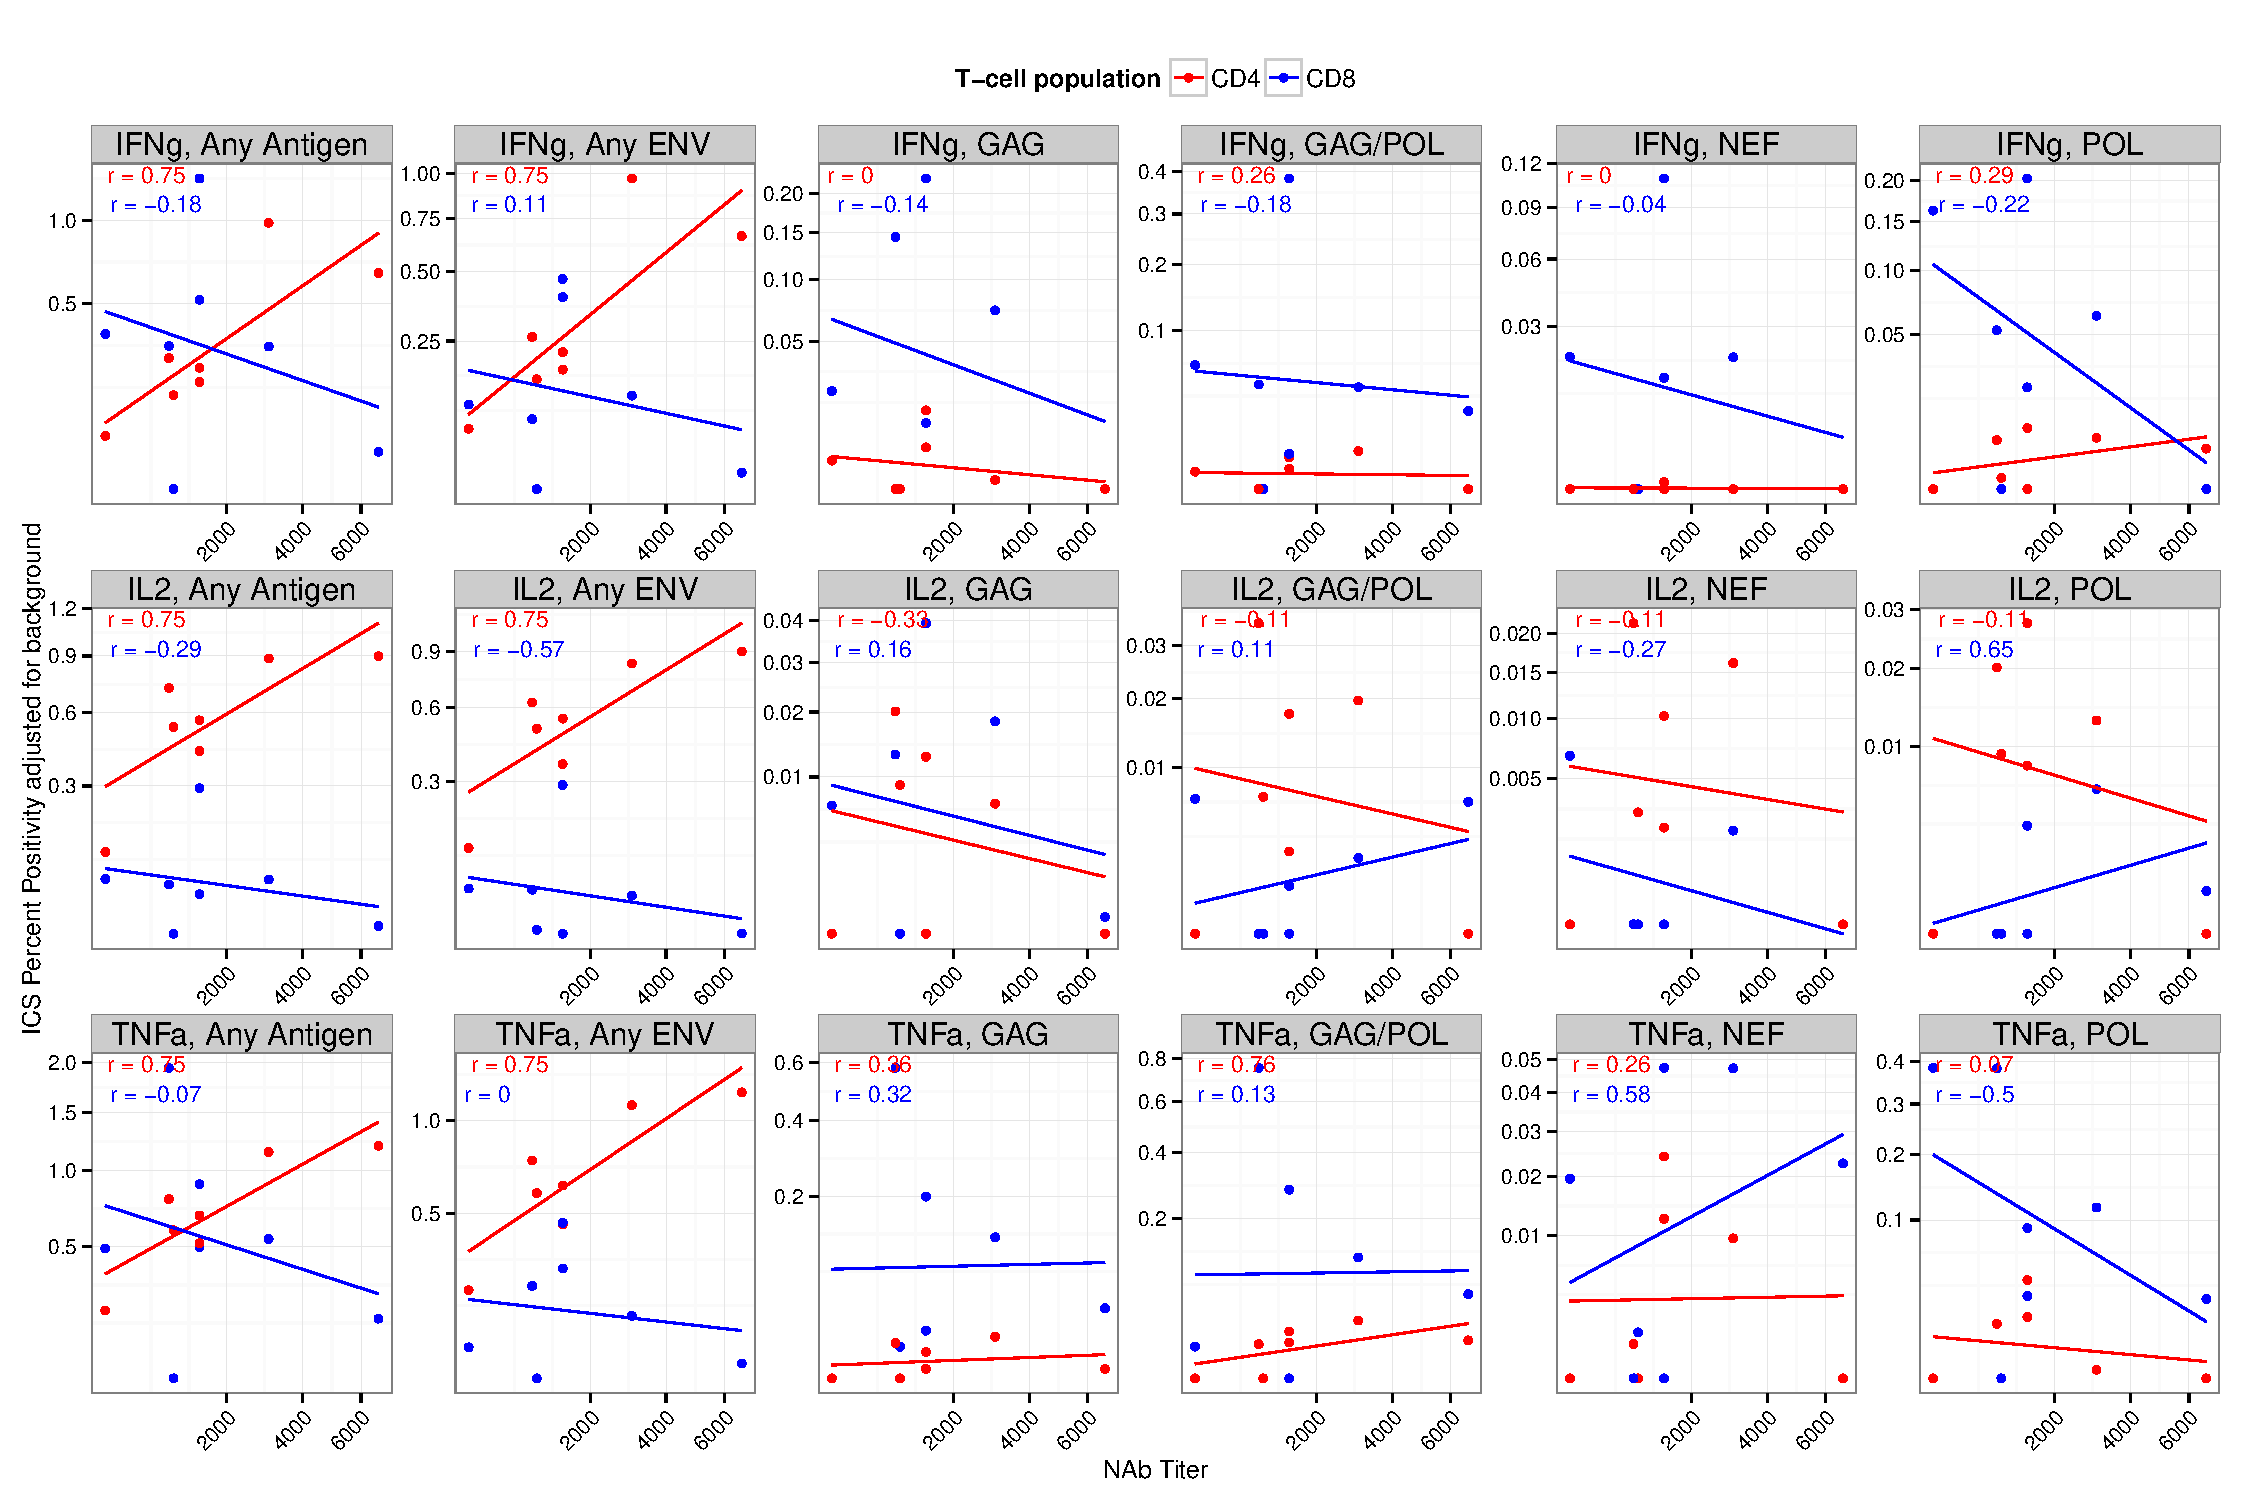
\includegraphics[width=\maxwidth]{figure/corrplot_Grp6_NAb_pooledAntigen-1} 

\end{knitrout}
\caption{Group 6, ICS v/s NAB assay by cytokine and pooled antigen colored by T-cell population. The fitted simple linear regression line and Spearman correlation are indicated.}
\end{center}
\end{figure}



% 
% \newpage
% <<dataprep,echo=FALSE,message=FALSE,warning=FALSE,error=FALSE>>=
% library(devtools)
% library(ggplot2)
% library(grid)
% library(gtools)
% library(reshape2)
% library(plyr)
% devtools::install_github("VIDD-VISC/AUP513", host="github.fhcrc.org/api/v3")
% rm(list=ls(all=TRUE))
% # Load data and R packages
% library(AUP513)
% data(AUP513_ics)
% data(AUP513_ics_marginal)
% data(AUP513_ics_marginal_pooled_across_antigen)
% data(AUP513_ics_pooled_across_cytokine)
% data(AUP513_ics_pooled_across_cytokine_antigen)
% 
% data(AUP513_bama)
% data(AUP513_adcc_gtl)
% data(AUP513_nab)
% #data(AUP513_elispot)
% 
% # # ICS data
% # datics <- AUP513_ics
% # table(datics$week)
% # datics <- datics[datics$week=="WK26",]
% # datics4 <- datics[datics$tcellsub=="CD4",]
% # datics4 <- datics4[datics4$antigen=="ENV1",]
% 
% # ICS marginal data
% daticsm <- AUP513_ics_marginal
% # table(daticsm$week)
% # daticsm <- daticsm[daticsm$week=="WK26" & daticsm$tcellsub=="CD4" & daticsm$antigen=="ENV1" & daticsm$cytokine=="IFNg",]
% daticsm <- daticsm[daticsm$week=="WK26",]
% daticsm <- daticsm[,c("ptid","group","week","antigen","tcellsub","cytokine","pctpos_adj")]
% colnames(daticsm) <- interaction("ics", colnames(daticsm))
% 
% # BAMA data
% datbama <- AUP513_bama
% # table(datbama$visitno)
% datbama <- datbama[datbama$visitno=="26" & datbama$isotype=="IgG" & datbama$antigen=="gp120 TV1",]
% datbama <- datbama[, c("isotype","ptid","visitno","antigen","dilution","auc_calculated")]
% colnames(datbama) <- interaction("bama", colnames(datbama))
% 
% # GTL data
% datgtl <- AUP513_adcc_gtl
% # table(datgtl$week)
% datgtl <- datgtl[datgtl$week=="26" & datgtl$antigen=="TV-1",]
% datgtl$log10titer <- log10(datgtl$titer)
% datgtl <- datgtl[!is.na(datgtl$log10titer),]
% datgtl <- datgtl[,c("antigen","ptid","group","week","log10titer")]
% colnames(datgtl) <- interaction("gtl", colnames(datgtl))
% 
% # NAB data
% datnab <- AUP513_nab
% # table(datnab$visitno)
% datnab <- datnab[datnab$visitno=="26" & datnab$celltype=="TZM-bl" & datnab$isolate=="MW965.26",]
% datnab <- datnab[,c("celltype","ptid","isolate","visitno","titer_mod")]
% colnames(datnab) <- interaction("nab", colnames(datnab))
% 
% # Merge all
% dat <- merge(daticsm, datbama, by.x="ics.ptid", by.y="bama.ptid", all=T)
% dat <- merge(dat, datgtl, by.x="ics.ptid", by.y="gtl.ptid", all=T)
% dat <- merge(dat, datnab, by.x="ics.ptid", by.y="nab.ptid", all=T)
% dat <- dat[!is.na(dat$ics.tcellsub) & !is.na(dat$bama.auc_calculated) & !is.na(dat$gtl.log10titer) & !is.na(dat$nab.titer_mod),]
% 
% datTot <- dat
% @
% % {\scriptsize
% % \tab \textbf{Footnote: \newline}
% % \tab *  -- Percentages in this group are computed using total number not enrolled as denominator. \newline
% % \tab ** -- Percent enrolled is computed as fraction of N screened. Subsequent percentages in this group are computed as a fraction of N enrolled.\newline
% % }
% 
% 
% 
% \begin{figure}[H]
% \begin{center}
% <<corrplot_Grp5_BAMA,fig.width=15,fig.height=10, echo=FALSE, warning=FALSE, cache=FALSE>>=
% # CD4 and CD8
% dat <- datTot[datTot$ics.group==5,]
% dat$response <- dat$bama.auc_calculated
% corsCD4 <- ddply(dat[dat$ics.tcellsub=="CD4",], c("ics.antigen","ics.cytokine","ics.tcellsub"), summarise, cor = round(cor(ics.pctpos_adj, response, method="spearman"), 2))
% corsCD8 <- ddply(dat[dat$ics.tcellsub=="CD8",], c("ics.antigen","ics.cytokine","ics.tcellsub"), summarise, cor = round(cor(ics.pctpos_adj, response, method="spearman"), 2))
% 
% ggplot(dat, aes(x=response, y=ics.pctpos_adj, colour=ics.tcellsub)) + theme_bw() +
%   xlab("BAMA AUC") +
%   ylab("ICS Percent Positivity adjusted for background") +
%   facet_grid(ics.cytokine ~ ics.antigen) + 
%   geom_point() +    
%   scale_colour_manual(name="T-cell population", values=c("CD4"="red", "CD8"="blue")) +
%   geom_text(data=corsCD4, size=4, aes(label=paste("r =", cor, sep=" ")), x=56000, y=0.7, color="red") + 
%   geom_text(data=corsCD8, size=4, aes(label=paste("r =", cor, sep=" ")), x=56000, y=0.6, color="blue") + 
%   geom_smooth(method=lm, se=FALSE)  +  # Don't add shaded confidence region
%   theme(#plot.margin = unit(c(1,1,0,1), "cm"),
%     legend.position="top",
%     legend.title=element_text(size=12,vjust=-1.6),
%     legend.text=element_text(size=12,vjust=-1.6),
%     axis.text.x = element_text(size=10, angle=45, hjust=1),
%     axis.text.y = element_text(size=10),
%     strip.text.x = element_text(size=15),
%     strip.text.y = element_text(size=15)) 
% @
% \caption{Group 5, ICS v/s BAMA by antigen and cytokine colored by T-cell population. The fitted simple linear regression line and Spearman correlation are indicated.}
% \end{center}
% \end{figure}
% 
% 
% \begin{figure}[H]
% \begin{center}
% <<corrplot_Grp5_ADCC,fig.width=15,fig.height=10, echo=FALSE, warning=FALSE, cache=FALSE>>=
% # CD4 and CD8
% dat <- datTot[datTot$ics.group==5,]
% dat$response <- dat$gtl.log10titer
% corsCD4 <- ddply(dat[dat$ics.tcellsub=="CD4",], c("ics.antigen","ics.cytokine","ics.tcellsub"), summarise, cor = round(cor(ics.pctpos_adj, response, method="spearman"), 2))
% corsCD8 <- ddply(dat[dat$ics.tcellsub=="CD8",], c("ics.antigen","ics.cytokine","ics.tcellsub"), summarise, cor = round(cor(ics.pctpos_adj, response, method="spearman"), 2))
% 
% ggplot(dat, aes(x=response, y=ics.pctpos_adj, colour=ics.tcellsub)) + theme_bw() +
%   xlab("GTL Log10 Titer") +
%   ylab("ICS Percent Positivity adjusted for background") +
%   facet_grid(ics.cytokine ~ ics.antigen) + 
%   geom_point() +    
%   scale_colour_manual(name="T-cell population", values=c("CD4"="red", "CD8"="blue")) +
%   geom_text(data=corsCD4, size=4, aes(label=paste("r =", cor, sep=" ")), x=3.5, y=0.8, color="red") + 
%   geom_text(data=corsCD8, size=4, aes(label=paste("r =", cor, sep=" ")), x=3.5, y=0.68, color="blue") + 
%   geom_smooth(method=lm, se=FALSE)  +  # Don't add shaded confidence region
%   theme(#plot.margin = unit(c(1,1,0,1), "cm"),
%     legend.position="top",
%     legend.title=element_text(size=12,vjust=-1.6),
%     legend.text=element_text(size=12,vjust=-1.6),
%     axis.text.x = element_text(size=10, angle=45, hjust=1),
%     axis.text.y = element_text(size=10),
%     strip.text.x = element_text(size=15),
%     strip.text.y = element_text(size=15)) 
% @
% \caption{Group 5, ICS v/s ADCC GTL assay by antigen and cytokine colored by T-cell population. The fitted simple linear regression line and Spearman correlation are indicated.}
% \end{center}
% \end{figure}
% 
% 
% \begin{figure}[H]
% \begin{center}
% <<corrplot_Grp5_NAb,fig.width=15,fig.height=10, echo=FALSE, warning=FALSE, cache=FALSE>>=
% # CD4 and CD8
% dat <- datTot[datTot$ics.group==5,]
% dat$response <- dat$nab.titer_mod
% corsCD4 <- ddply(dat[dat$ics.tcellsub=="CD4",], c("ics.antigen","ics.cytokine","ics.tcellsub"), summarise, cor = round(cor(ics.pctpos_adj, response, method="spearman"), 2))
% corsCD8 <- ddply(dat[dat$ics.tcellsub=="CD8",], c("ics.antigen","ics.cytokine","ics.tcellsub"), summarise, cor = round(cor(ics.pctpos_adj, response, method="spearman"), 2))
% 
% ggplot(dat, aes(x=response, y=ics.pctpos_adj, colour=ics.tcellsub)) + theme_bw() +
%   xlab("NAb Titer") +
%   ylab("ICS Percent Positivity adjusted for background") +
%   facet_grid(ics.cytokine ~ ics.antigen) + 
%   geom_point() +    
%   scale_colour_manual(name="T-cell population", values=c("CD4"="red", "CD8"="blue")) +
%   geom_text(data=corsCD4, size=4, aes(label=paste("r =", cor, sep=" ")), x=5000, y=0.8, color="red") + 
%   geom_text(data=corsCD8, size=4, aes(label=paste("r =", cor, sep=" ")), x=5000, y=0.7, color="blue") + 
%   geom_smooth(method=lm, se=FALSE)  +  # Don't add shaded confidence region
%   theme(#plot.margin = unit(c(1,1,0,1), "cm"),
%     legend.position="top",
%     legend.title=element_text(size=12,vjust=-1.6),
%     legend.text=element_text(size=12,vjust=-1.6),
%     axis.text.x = element_text(size=10, angle=45, hjust=1),
%     axis.text.y = element_text(size=10),
%     strip.text.x = element_text(size=15),
%     strip.text.y = element_text(size=15)) 
% @
% \caption{Group 5, ICS v/s NAB assay by antigen and cytokine colored by T-cell population. The fitted simple linear regression line and Spearman correlation are indicated.}
% \end{center}
% \end{figure}
% 
% 
% 
% \begin{figure}[H]
% \begin{center}
% <<corrplot_Grp6_BAMA,fig.width=15,fig.height=10, echo=FALSE, warning=FALSE, cache=FALSE>>=
% # CD4 and CD8
% dat <- datTot[datTot$ics.group==6,]
% dat$response <- dat$bama.auc_calculated
% corsCD4 <- ddply(dat[dat$ics.tcellsub=="CD4",], c("ics.antigen","ics.cytokine","ics.tcellsub"), summarise, cor = round(cor(ics.pctpos_adj, response, method="spearman"), 2))
% corsCD8 <- ddply(dat[dat$ics.tcellsub=="CD8",], c("ics.antigen","ics.cytokine","ics.tcellsub"), summarise, cor = round(cor(ics.pctpos_adj, response, method="spearman"), 2))
% 
% ggplot(dat, aes(x=response, y=ics.pctpos_adj, colour=ics.tcellsub)) + theme_bw() +
%   xlab("BAMA AUC") +
%   ylab("ICS Percent Positivity adjusted for background") +
%   facet_grid(ics.cytokine ~ ics.antigen) + 
%   geom_point() +    
%   scale_colour_manual(name="T-cell population", values=c("CD4"="red", "CD8"="blue")) +
%   geom_text(data=corsCD4, size=4, aes(label=paste("r =", cor, sep=" ")), x=52000, y=0.7, color="red") + 
%   geom_text(data=corsCD8, size=4, aes(label=paste("r =", cor, sep=" ")), x=52000, y=0.65, color="blue") + 
%   geom_smooth(method=lm, se=FALSE)  +  # Don't add shaded confidence region
%   theme(#plot.margin = unit(c(1,1,0,1), "cm"),
%     legend.position="top",
%     legend.title=element_text(size=12,vjust=-1.6),
%     legend.text=element_text(size=12,vjust=-1.6),
%     axis.text.x = element_text(size=10, angle=45, hjust=1),
%     axis.text.y = element_text(size=10),
%     strip.text.x = element_text(size=15),
%     strip.text.y = element_text(size=15)) 
% @
% \caption{Group 6, ICS v/s BAMA by antigen and cytokine colored by T-cell population. The fitted simple linear regression line and Spearman correlation are indicated.}
% \end{center}
% \end{figure}
% 
% 
% \begin{figure}[H]
% \begin{center}
% <<corrplot_Grp6_ADCC,fig.width=15,fig.height=10, echo=FALSE, warning=FALSE, cache=FALSE>>=
% # CD4 and CD8
% dat <- datTot[datTot$ics.group==6,]
% dat$response <- dat$gtl.log10titer
% corsCD4 <- ddply(dat[dat$ics.tcellsub=="CD4",], c("ics.antigen","ics.cytokine","ics.tcellsub"), summarise, cor = round(cor(ics.pctpos_adj, response, method="spearman"), 2))
% corsCD8 <- ddply(dat[dat$ics.tcellsub=="CD8",], c("ics.antigen","ics.cytokine","ics.tcellsub"), summarise, cor = round(cor(ics.pctpos_adj, response, method="spearman"), 2))
% 
% ggplot(dat, aes(x=response, y=ics.pctpos_adj, colour=ics.tcellsub)) + theme_bw() +
%   xlab("GTL Log10 Titer") +
%   ylab("ICS Percent Positivity adjusted for background") +
%   facet_grid(ics.cytokine ~ ics.antigen) + 
%   geom_point() +    
%   scale_colour_manual(name="T-cell population", values=c("CD4"="red", "CD8"="blue")) +
%   geom_text(data=corsCD4, size=4, aes(label=paste("r =", cor, sep=" ")), x=3.5, y=0.8, color="red") + 
%   geom_text(data=corsCD8, size=4, aes(label=paste("r =", cor, sep=" ")), x=3.5, y=0.75, color="blue") + 
%   geom_smooth(method=lm, se=FALSE)  +  # Don't add shaded confidence region
%   theme(#plot.margin = unit(c(1,1,0,1), "cm"),
%     legend.position="top",
%     legend.title=element_text(size=12,vjust=-1.6),
%     legend.text=element_text(size=12,vjust=-1.6),
%     axis.text.x = element_text(size=10, angle=45, hjust=1),
%     axis.text.y = element_text(size=10),
%     strip.text.x = element_text(size=15),
%     strip.text.y = element_text(size=15)) 
% @
% \caption{Group 6, ICS v/s ADCC GTL assay by antigen and cytokine colored by T-cell population. The fitted simple linear regression line and Spearman correlation are indicated.}
% \end{center}
% \end{figure}
% 
% 
% \begin{figure}[H]
% \begin{center}
% <<corrplot_Grp6_NAb,fig.width=15,fig.height=10, echo=FALSE, warning=FALSE, cache=FALSE>>=
% # CD4 and CD8
% dat <- datTot[datTot$ics.group==6,]
% dat$response <- dat$nab.titer_mod
% corsCD4 <- ddply(dat[dat$ics.tcellsub=="CD4",], c("ics.antigen","ics.cytokine","ics.tcellsub"), summarise, cor = round(cor(ics.pctpos_adj, response, method="spearman"), 2))
% corsCD8 <- ddply(dat[dat$ics.tcellsub=="CD8",], c("ics.antigen","ics.cytokine","ics.tcellsub"), summarise, cor = round(cor(ics.pctpos_adj, response, method="spearman"), 2))
% 
% ggplot(dat, aes(x=response, y=ics.pctpos_adj, colour=ics.tcellsub)) + theme_bw() +
%   xlab("NAb Titer") +
%   ylab("ICS Percent Positivity adjusted for background") +
%   facet_grid(ics.cytokine ~ ics.antigen) + 
%   geom_point() +    
%   scale_colour_manual(name="T-cell population", values=c("CD4"="red", "CD8"="blue")) +
%   geom_text(data=corsCD4, size=4, aes(label=paste("r =", cor, sep=" ")), x=5000, y=0.8, color="red") + 
%   geom_text(data=corsCD8, size=4, aes(label=paste("r =", cor, sep=" ")), x=5000, y=0.75, color="blue") + 
%   geom_smooth(method=lm, se=FALSE)  +  # Don't add shaded confidence region
%   theme(#plot.margin = unit(c(1,1,0,1), "cm"),
%     legend.position="top",
%     legend.title=element_text(size=12,vjust=-1.6),
%     legend.text=element_text(size=12,vjust=-1.6),
%     axis.text.x = element_text(size=10, angle=45, hjust=1),
%     axis.text.y = element_text(size=10),
%     strip.text.x = element_text(size=15),
%     strip.text.y = element_text(size=15)) 
% @
% \caption{Group 6, ICS v/s NAB assay by antigen and cytokine colored by T-cell population. The fitted simple linear regression line and Spearman correlation are indicated.}
% \end{center}
% \end{figure}





\end{landscape}
\end{document}
